\documentclass[tikz,border=2pt]{standalone}
\usetikzlibrary{arrows.meta,positioning,calc}
\definecolor{paper}{HTML}{EFE8D8}
\definecolor{ink}{HTML}{2B2A28}
\definecolor{ground}{HTML}{D9CDB2}
\definecolor{muted}{HTML}{6B6457}
\definecolor{cond}{HTML}{3E4A89}
\definecolor{act}{HTML}{7A5618}
\input{/Users/samgilson/Documents/vagrancy/analysis/trees/icons.tex}
\begin{document}
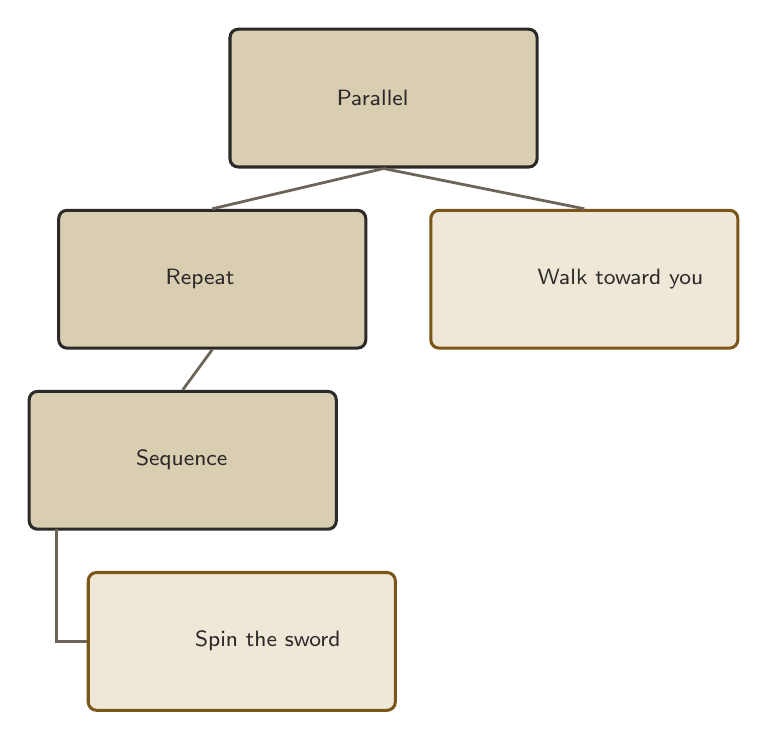
\begin{tikzpicture}[font=\sffamily,
  box/.style={draw, line width=1.1pt, rounded corners=3pt, minimum width=3.9cm, minimum height=1.75cm},
  comp/.style={draw=ink, fill=ground}, cond/.style={draw=cond, fill=paper}, act/.style={draw=act, fill=paper},
  srch/.style={draw=cond, fill=paper, line width=2pt},
  label/.style={anchor=west, text=ink, text width=2.30cm, align=left, font=\sffamily\footnotesize, inner sep=0pt},
  edge/.style={draw=muted, line width=1pt}]
% --- Nodes ---
\node[box, comp] (n0) at (4.500,-0.875) {};
\begin{scope}[shift={(2.800,-1.350)}, x=0.0950cm, y=0.0950cm]\def\IC{ink}\def\IW{0.7pt}\IconParallel\end{scope}
\node[label] at (3.900,-0.875) {Parallel};
\node[box, comp] (n1) at (2.325,-3.175) {};
\begin{scope}[shift={(0.625,-3.650)}, x=0.0950cm, y=0.0950cm]\def\IC{ink}\def\IW{0.7pt}\IconRepeat\end{scope}
\node[label] at (1.725,-3.175) {Repeat};
\node[box, comp] (n2) at (1.950,-5.475) {};
\begin{scope}[shift={(0.250,-5.950)}, x=0.0950cm, y=0.0950cm]\def\IC{ink}\def\IW{0.7pt}\IconSequence\end{scope}
\node[label] at (1.350,-5.475) {Sequence};
\node[box, act] (n3) at (2.700,-7.775) {};
\begin{scope}[shift={(1.000,-8.250)}, x=0.0950cm, y=0.0950cm]\def\IC{ink}\def\IW{0.7pt}\IconSpin\end{scope}
\node[label] at (2.100,-7.775) {Spin the sword};
\node[box, act] (n4) at (7.050,-3.175) {};
\begin{scope}[shift={(5.350,-3.650)}, x=0.0950cm, y=0.0950cm]\def\IC{ink}\def\IW{0.7pt}\IconApproach\end{scope}
\node[label] at (6.450,-3.175) {Walk toward you};
% --- Edges (after the nodes they join; they end at the borders) ---
\draw[edge] (0.350,-6.350) |- (n3.west);
\draw[edge] (n1.south) -- (n2.north);
\draw[edge] (n0.south) -- (n1.north);
\draw[edge] (n0.south) -- (n4.north);
\end{tikzpicture}
\end{document}
